\input{../common}

\begin{document}
  %<*content>
  \lesson{analysis}{25}{Fonction  logarithme népérien (TL)}
  
  
Avant l'invention des calculateurs (ordinateurs, calculatrices, ...) les mathématiciens ont cherché à simplifier les calculs à effectuer.

\medskip
1) Durant l'Antiquité (IIIème siècle avant J.C.), Archimède avait remarqué que pour multiplier certains nombres, il suffisait de savoir additionner! et qu'il était plus facile d'effectuer des additions plutôt que des multiplications! 

\medskip

2) John Napier (ou Neper), baron écossais (1550-1617), a repris et étendu l'idée d'Archimède et a mis au point une méthode générale qui permet d'effectuer

-des additions à la place de multiplications

-des soustractions à la place de divisions;

ce sont les \textbf{logarithmes.}

\medskip
3) Modéliser la forme d'un cyclone, d'un coquillage  ou d'une fleur de tournesol, mais aussi représenter sur un même graphique  les distances des planètes en fonction de leurs périodes  de révolution , sont autant d'activités qui utilisent une même famille de fonctions: les logarithmes. 
 
 \subsection{Définition et propriétés}
\begin{definition}
 On appelle fonction logarithme népérien,  notée $ \ln$ ,\; la fonction  dérivable sur $ \intoo{0}{\pinf} $ qui a pour   fonction   dérivée \;$ x  \longmapsto \dfrac{1}{x} $ \; et  qui s'annule pour \; $ x=1 $.
\end{definition}

\begin{example}[calcul à l'aide  de la calculatrice]

$$\begin{array}{|c|c|c|c|c|c|c|c|c|c|c|}
\hline
 x & -3&  -1 &  0 &  0.2  &0.5 &  1 &  2  &  8  &  50  & 100 \\
\hline
 \ln x   &  \times  &  \times  &  \times  &  - 1,609 &  - 0,693 & 0&  0,693 &2,079 &3,912 &4,605\\
\hline

\end{array}$$


\end{example}
\begin{corollary}
\begin{enumerate}
\item Le domaine de définition de la fonction $ \ln $  est  $ \intoo{0}{\pinf} $.
\item La fonction $ \ln $  est  dérivable  sur  $ \intoo{0}{\pinf} $  et pour tout $ x> 0 $ on a \quad  \fbox{  $\ln'(x)=\dfrac{1}{x} $ }.
\item \fbox{$\ln (1)= 0$ }.
\item  La dérivée de la fonction $ \ln $ étant strictement positive  sur $ \intoo{0}{\pinf} $, donc la  fonction $ \ln $  est strictement croissante sur  $ \intoo{0}{\pinf} $.
\end{enumerate}
\end{corollary}
\begin{property}
\begin{align*}
    \text{Pour tous} \;a > 0 \;  \text{et} \;b > 0 ,\quad & a< b \Longleftrightarrow \ln a < \ln b \\
    & a> b \Longleftrightarrow \ln a  >\ln b  \\
    & a= b \Longleftrightarrow \ln a  =\ln b
    \end{align*} 
   \end{property}
  \begin{property}[Propriété fondamentale]
 $$\text{Pour tous}\quad  a> 0 \quad  \text{ et} \quad  b>0 ,\;\text{ on a }\quad  \ln(ab)=\ln a +\ln b $$

   \end{property}
\begin{corollary}[propriétés algébriques]
Soient $ a > 0$  et  $ b > 0$.
\begin{enumerate}
\item[\textbullet] $  \ln \paren{\dfrac{1}{a}}= - \ln a$
\item[\textbullet] $\ln \paren{\dfrac{a}{b} }= \ln a-  \ln b$
 \item[\textbullet] $  \ln \sqrt{a} = \frac{1}{2} \ln a$
 \item[\textbullet] $ \ln a^{n} = n\ln a \quad \text{pour tout} \;  n\in\Qq$
\end{enumerate}
\end{corollary}
\subsection{ Étude de la fonction ln }

 \begin{property}[Limites]
 $ \bullet \; \displaystyle\lim_{x \to \pinf}\ln x=\pinf  \hspace*{4cm}    \bullet  \; \displaystyle\lim_{x \to 0^{+}}\ln x=\minf $
  \end{property}
  

\textbf{Tableau de variation }\\
Des propriétés précédentes, on en déduit  le tableau de variation suivant.

\begin{center}

\begin{tikzpicture}
\tkzTabInit[lgt=2, espcl=3]%
{$x$ / 1 , $\ln'(x)$ / 1 , $\ln(x)$ / 2}%
{$0$, $+\infty$}

\tkzTabLine{ , + , }
\tkzTabVar{-/$-\infty$, +/$+\infty$}
\end{tikzpicture}

\end{center}
\begin{corollary}
La fonction $ \ln  $  est continue et strictement croissante sur $ \intoo{0}{\pinf} $  cela entraîne que c'est une bijection de $ \intoo{0}{\pinf} $  vers $ \Rr $.

Donc  pour tout  $  y \in \Rr $, \; il existe un unique $ x\in \intoo{0}{\pinf} $ tel que $ \ln x=y. $ 

 En particulier il existe un unique réel noté $ \mathrm{e} $ tel que: \quad \fbox { $\ln \mathrm{e}=1 $}.\\

On démontre que $ \mathrm{e}\simeq 2,718 $,    il  est appelé la   {\bf  constante d' Euler}.\\

On a alors  pour tout $  n \in \Qq, \; \ln \eexp{n}=n\ln \mathrm{e}=n $\\


Ainsi:
\medskip

$\begin{array}{ |l|c|r|}
\hline
 \ln x = n  \Longleftrightarrow x = \eexp{n} &
 \ln x  > n \Longleftrightarrow x   >\eexp{n} &
 \ln x  < n\Longleftrightarrow x <   \eexp{n} \\
\hline
\end{array}$

\end{corollary}
\subsection*{Représentation graphique de la fonction $ \ln $}

On construit les tangentes  T$ _{1} $   et T$ _{2} $ à la courbe de $ \ln $   respectives  aux points  d'abscisses $ x=1$ et $x= \mathrm{e} $.

 T$ _{1} \;: y= \ln'(1)(x-1) +\ln1$ \; soit \; T$ _{1}:\;y=x-1 $ 
 
  T$ _{2} \;: y= \ln'(\mathrm{e})(x-\mathrm{e}) +\ln \mathrm{e}$ \; soit \; T$ _{2}:\;y=\tfrac{1}{\mathrm{e}}x $ 
 
 
\begin{tikzpicture}[>=stealth', scale=0.5]
\clip (-2,-3) rectangle (8,4);
\draw[->,thick] (0,0) -- (1,0);
\draw[->,thick] (0,0) -- (0,1);
\draw[,thick] (-2,0) -- (8,0);
\draw[thick] (0,-3) -- (0,4);
\foreach\x in {1,2,}
{
\draw[thick] (\x,0.1) -- (\x,-0.1) node[below] {\x};
}
\foreach\y in {1}
{
\draw[thick] (0.1,\y) -- (-0.1,\y) node[left] {\y};
}

\draw[thick,red] plot[domain=0.01 :7,samples=100] (\x,{ln (\x)}) node[below right] {$\mathscr{C}$};
\draw[thick,green] plot[domain=-1 :6,samples=100] (\x,{\x-1}) node[below  left] {$T_{1}$};
\draw[thick,green] plot[domain=-1 :6,samples=100] (\x,{0.4*\x}) node[below  left] {};
\draw[dashed,thick](2.7,0)--(2.7,1);
\draw[dashed,thick](2.7,1)--(0,1);
\node at(2.7,-0.4) {$\mathrm{e}$};
\node at(7,2.6) {$T_{2} $};
\node at(4.5,3) {$T_{1} $};
\end{tikzpicture}

\fbox{$ \displaystyle\lim_{x \to 0^{+}}x\ln x=0 \hspace*{1cm} \lim_{x \to \pinf}\dfrac{\ln x}{x}=0 $}

\subsection*{Equations, inéquations et systèmes}
\textbf{Equations comportant ln}\\
\textbf{methode}\\
Pour résoudre une équation comportant des logarithmes,
\begin{itemize}
\item[$ \bullet$] on détermine le domaine D de résolution;
\item[$ \bullet$] on transforme si possible l'équation sous la forme $ \ln A=\ln B $;
\item[$ \bullet$] résout l'équation $ A=B $;
\item[$ \bullet$]  puis on retient que les solutions appartenant à D.
\end{itemize}
\begin{example} Résoudre dans $ \Rr $ l'équation: $\quad \ln (2x-3)-\ln x=0 $

L'équation est définie lorsque $2x-3>0$ et $ x>0$  c'est-à-dire $ x>\frac{3}{2}.\quad$ Ainsi D$ =\intoo{\frac{3}{2}}{\pinf} $.

L'équation devient  $ \ln (2x-3)=\ln x$  ce qui équivaut à $ 2x-3=x $  soit $ x=3 $ qui est bien dans D. Donc S$ =\accol{3} $
\end{example}
\begin{example} Résoudre dans $ \Rr $ l'équation : $\; \ln (x+5)+\ln (x+3)=\ln15  $

L'équation est définie lorsque $x+5>0$ et $ x+2>0$  c'est-à-dire $ x>-5 $  et $ x>-3 $.\\   Ainsi D$ =\intoo{-3}{\pinf} $.

L'équation devient  $ \ln (x+5)(x+3)=\ln 15$ \\Ce qui équivaut à $ (x+5)(x+3)=15 $  soit $ x^{2}+8x+15=0 $  ou encore $ x^{2}+8x=0 $  soit $x=0 $ ou $x=-8\quad $
 Donc S$ =\accol{0} $
\end{example}

\textbf{Equations du type $a\ln^{2} x+b\ln x+c=0$ }\\
Poser $ \ln x=X $ puis résoudre l'équation E du second degré $ aX^{2}+bX+c=0 $ et enfin les équations $ \ln x=X_{1} $  et $ \ln x=X_{2} $  où $ X_{1}$ et $X_{2} $  sont les solutions de E.
\begin{example} Résolvons dans $ \Rr $  l'équation  :\; $ \paren{\ln x}^{2} -6\ln x+5=0 $. 

Pour $ x> 0 $, posons  $ \ln x=X $ ,\; l'équation  \; devient $ X^{2} -6X+5=0$ d'où $X=1 $ ou $X=5 $.

Ainsi  $ \ln x=1 \Longleftrightarrow x=\eexp{}$  ou $ \ln x=5 \Longleftrightarrow x=\eexp{5}$\; d'où S$ =\accol{\eexp{},\eexp{5}} $
\end{example}
\textbf{Inéquation comportant ln}\\
\textbf{methode}\\
Pour résoudre une inéquation comportant des logarithmes,
\begin{itemize}
\item[$ \bullet$] on détermine le domaine D de résolution;
\item[$ \bullet$] on transforme si possible l'inéquation sous la forme $ \ln A<\ln B $  ou $ \ln A\geq\ln B $;
\item[$ \bullet$] résout l'inéquation $ A< B $  ou $ A\geq B $;
\item[$ \bullet$]  puis on retient que les solutions appartenant à D.
\end{itemize}

\begin{example} Résoudre dans $ \Rr $ l'équation : $\; \ln (2x-3)-\ln x< 0 $.

L'inéquation est définie lorsque $2x-3>0$ et $ x>0$  c'est-à-dire $ x>\frac{3}{2}.\quad $ Ainsi D$ =\intoo{\frac{3}{2}}{\pinf} $.

L'inéquation devient  $ \ln (2x-3)<\ln x$  ce qui équivaut à $ 2x-3<x $  soit $ x<3 $ qui est bien dans D. Donc S$ =\intoo{\frac{3}{2}}{\pinf}\cap \intoo{\minf}{3}= \intoo{\frac{3}{2}}{3}$
\end{example}
\begin{example} Résoudre dans $ \Rr $ l'inéquation: $\; \ln (x+5)+\ln (x+3)\leq\ln 15  $


L'inéquation est définie lorsque $x+5>0$ et $ x+2>0$  c'est-à-dire $ x>-5 $  et $ x>-3 $.\\  Ainsi D$ =\intoo{-3}{\pinf} $.

L'inéquation devient  $ \ln (x+5)(x+3)\leq\ln 15$ \\Ce qui équivaut à $ (x+5)(x+3)\leq 15 $  soit $ x^{2}+8x+15\leq 0 $  ou encore $ x^{2}+8x\leq 0 $. 
%\renewcommand{\arraystretch}{1}
 \[
\begin{array}{|c|c|c|c|c|}
\hline
x & \minf < x < -8 & x = -8 & -8 < x < 0 & x > 0 \\
\hline
x^{2} + 8x & + & 0 & - & + \\
\hline
\end{array}
\]

  
 Donc S$ = \intoo{-3}{\pinf}\cap\intff{-8}{0}=\intof{-3}{0}$
\end{example}
\textbf{Systèmes d'équations comportant ln}
\begin{example}
Résolvons le système suivant.

\medskip

$  \left\{\begin{array}{l} 2\ln x+3\ln y=2 \\ 5\ln x-\ln y=22\end{array}\right.$

Le système est défini pour $x>0 $ et $y>0 $.

\medskip
En posant $X=\ln x  $ et $Y=\ln y,\; $  le système devient:
   $ \quad \left\{\begin{array}{l} 2X+3Y=2 \\ 5X-Y=22\end{array}\right.$

\medskip

En utilisant la méthode d'addition par exemple, on trouve $X=4 $ et $Y=-2 $.

\medskip
Puis $\ln x=4 \Longleftrightarrow  x=\eexp{4} $  et $\ln y=-2 \Longleftrightarrow  y=\eexp{-2} $ \\

D'où S$ =\accol{\paren{\eexp{4},\eexp{-2}},\paren{\eexp{-2},\eexp{4}}} $

\end{example}
\begin{example}
Résolvons le système suivant.

\medskip

$  \left\{\begin{array}{l} \ln x+\ln y=\ln 12  \\ \ln (x+y)=\ln 2+\ln 4 \end{array}\right.$

Le système est défini pour $x>0 $ et $y>0 $.

\medskip
On peut réécrire le système  sous la forme:
\medskip

$  \left\{\begin{array}{l} \ln xy=\ln 12  \\ \ln (x+y)=\ln 8 \end{array}\right.$
\quad soit   $  \left\{\begin{array}{l} xy=12 \\ x+y=8\end{array}\right.$

\medskip

Ainsi les réels $x $ et $y $ vérifient l'équation du second degré \; $ X^{2}-8X+12=0 $
\bigskip


On trouve $X_{1}=2  $  et $X_{2}=6$ \;d'où \;S$ =\accol{\paren{2,6},\paren{6,2}} $

\end{example}
\subsection{ Etude des fonctions faisant intervenir ln }
Soit $ u $ une fonction définie sur un intervalle I.

On considère la fonction $ f $ définie pour tout $ x\in I $ par : \; $ f(x)=\ln \paren{u(x)} $.\\\
\textbf{Domaine de définition}\\
$ f(x)  $ existe  si et seulement si $ u(x)>0 $
\begin{example}

$ f(x)=\ln \paren{x^{2}-1} $  existe  si et seulement si $ x^{2}-1>0 $ c'est-à-dire $ x<-1$ ou $ x>1 $


\medskip
$ Df=\intoo{\minf}{-1}\cup\intoo{1}{\pinf} $
\end{example}
\begin{remark}

$ \bullet $  Attention le domaine de définition de $ \ln u $  n'est pas  forcément celui de la fonction $ \ln x  $  de la définition initiale.

$ \bullet $\; $ f(x)=\ln \abs{u(x)} $  existe  si et seulement si $ u(x)\neq 0 $
\end{remark}

\begin{example}

$ f(x)=\ln \abs{\dfrac{x-3}{x-2}} $  existe  si et seulement si $ \dfrac{x-3}{x-2}\neq 0 $ si et seulement si $ x\neq3 $  et $ x\neq2 $ c'est-à-dire $ x\in\Rr\setminus \accol{2,3}.\quad  $ Ainsi 
$ Df=\intoo{\minf}{2}\cup \intoo{2}{3}\cup\intoo{3}{\pinf}$
\end{example}

\begin{property}[Limites]
\begin{itemize}
\item[$ \bullet $]  Si $ u  $ tend vers \textbf{$ L $}  alors $ \ln u $  tend vers \textbf{$\ln L$}. 
\item[$ \bullet $]  Si $ u  $ tend vers $ \pinf $  alors $ \ln u $  tend vers $ \pinf $.
\item[$ \bullet $]  Si $ u  $ tend vers $ 0^{+} $  alors $ \ln u $  tend vers $ \minf $.

\end{itemize}
\end{property}

\begin{example}
\begin{itemize}
\item[$ \bullet $] $ \limi{x}{\pinf}{\frac{x+3}{x-8}}=\limi{x}{\pinf}{\frac{x}{x}}=1 $ donc $ \limi{x}{\pinf}{\ln\paren{\frac{x+3}{x-8}} }=\ln 1=0$


\item[$ \bullet $] $ \limi{x}{\minf}{\dfrac{x+3}{x-8}}=\limi{x}{\minf}{\dfrac{x}{x}}=1 \;$ donc $ \;\limi{x}{\minf}{\ln\paren{\dfrac{x+3}{x-8}} }=\ln 1=0$



 \item[$ \bullet $]  $ \limi{x}{1^{+}}{x^{2}-1}=0^{+}\; $ donc $\; \limi{x}{1^{+}}{\ln\paren{x^{2}-1} }=\minf$
 
\item[$ \bullet $] $ \limi{x}{1^{-}}{x^{2}-1}=0^{+}\; $ donc $\; \limi{x}{1^{-}}{\ln\paren{x^{2}-1} }=\minf$
\end{itemize}
\end{example}

\textbf{Dérivée}\\
Nous admettons le théorème suivant.
\begin{theorem}
\begin{itemize}
\item[$ \bullet \;$] Si  $\; u $  est  une fonction dérivable et strictement positive sur un intervalle I alors la fonction  $ \; \ln u $ est dérivable sur I et on a:  $ \paren{\ln u}^{\prime}=\dfrac{u^{\prime}}{u} $
\item[$ \bullet $] Si  $ \; u $  est  une fonction dérivable et non nulle sur un intervalle I alors la fonction  $\;  \ln \abs{u} $ est dérivable sur I et on a:  $ \paren{\ln \abs{u}}^{\prime}=\dfrac{u^{\prime}}{u} $
\end{itemize}
\end{theorem}

\begin{example}
\begin{itemize}
\item[$ \bullet \;$]  La fonction $ x\longmapsto 2x-1 $  est dérivable et strictement positive sur 
$ \intoo{\dfrac{1}{2}}{\pinf} \; $ donc la fonction $\;  x\longmapsto \ln \paren{2x-1 }\; $ est dérivable sur $_; \intoo{\frac{1}{2}}{\pinf} \;$ et pour tout $\;  x> \frac{1}{2},\; $ on a: $\;   \ln^{\prime} \paren{2x-1 } =\dfrac{2}{2x-1} $.

\item[$ \bullet \;$] Soit $ f $ la fonction  définie par $ f(x)= \ln \paren{{x^2} + 3x - 4 } $

$\ln \paren{{x^2} + 3x - 4 }$ existe  si et seulement si
    ${x^2} + 3x - 4 > 0$.

    On recherche les racines de $u\left( x \right) = {x^2} + 3x - 4$.

    $\Delta = {3^2} - 4 \times 1\left( { - 4} \right) = 25 =
    {5^2}\; $. 
  Le trin\^{o}me a deux racines~: 
  $\;{x_1} = \dfrac{{ - 3 - 5}}{2} = - 4{\text{ et }}{x_2} = \dfrac{{
        - 3 + 5}}{2} = 1$.
        
        $u\left( x \right)$ est du signe de $a = 1$, soit positif sauf
    entre les racines.
    
    Donc $f$ est bien définie sur $\left] {-\infty\ ;\ - 4} \right[
    \cup \left] {1\ ;\ + \infty } \right[$.
    
    $ u $   est dérivable ( car polynôme) et   strictement positive sur $\left] {-\infty\ ;\ - 4} \right[
    \cup \left] {1\ ;\ + \infty } \right[$.
    
Donc    $ f^{\prime}(x)=\ln^{\prime} \paren{{x^2} + 3x - 4 } =\dfrac{2x+3}{{x^2} + 3x - 4}$

 \end{itemize}
\end{example}
  %</content>
\end{document}
